\section{Results}

\subsection{Miss-use modeling}

\begin{table}[h!]
\centering
  \caption{Summary of cascades level population.}
\begin{tabular}{ccccccccc}
\toprule

Model       &        &           & A/NR      & A/R       & B/NR      & B/R      & C/NR       & C/R          \\
%Recycling   &        &           & No        & yes       & No        & Yes     & No        & yes        \\
\midrule                                                                                                 
        &            & Feed      & $0.71w\%$ & $1.3w\%$  & $0.71w\%$ & $0.94w\%$ & $0.71w\%$ & $1.66w\%$ \\
Level 0 & Assay      & Product   & $4.13w\%$ & $7.7w\%$  & $4.13w\%$ & $5.43w\%$ & $4.13w\%$ & $9.53w\%$ \\
        &            & Tails     & $0.29w\%$ & $0.5w\%$  & $0.29w\%$ & $0.39w\%$ & $0.29w\%$ & $0.69w\%$ \\
        & Cascades   &           & 25        & 25        & 25        & 24        & 25        & 25        \\
\midrule                                                                                                 
        &            & Feed      & $4.13w\%$ & $11.9w\%$ & $4.13w\%$ & $6.84w\%$ & $4.13w\%$ & $13.0w\%$ \\
Level 1 & Assay      & Product   & $22.8w\%$ & $55.7w\%$ & $20.6w\%$ & $30.7w\%$ & $22.9w\%$ & $69.8w\%$ \\
        &            & Tails     & $1.8w\%$  & $6.6w\%$  & $1.72w\%$ & $2.91w\%$ & $1.81w\%$ & $9.43w\%$ \\
        & Cascades   &           & 3         & 4         & 3         & 4         & 3         & 4         \\
\midrule                                                                                                 
        &            & Feed      & $22.8w\%$ & $55.7w\%$ & $20.6w\%$ & $34.3w\%$ & $22.9w\%$ & $72.6w\%$ \\
Level 2 & Assay      & Product   & $78.5w\%$ & $95.0w\%$ & $61.0w\%$ & $75.8w\%$ & $82.0w\%$ & $98.4w\%$ \\
        &            & Tails     & $4.12w\%$ & $50.9w\%$ & $9.56w\%$ & $17.5w\%$ & $15.7w\%$ & $69.4w\%$ \\
        & Cascades   &           & 1         & 1         & 1         & 1         & 1         & 1         \\
\midrule                                                                                                 
        &            & Feed      & $78.5w\%$ & N.A.      & $61.0w\%$ & $75.8w\%$ & $82.3w\%$ & N.A.      \\
Level 3 & Assay      & Product   & $98.2w\%$ & N.A.      & $90.4w\%$ & $95.0w\%$ & $99.1w\%$ & N.A.      \\
        &            & Tails     & $76.1w\%$ & N.A.      & $79.3w\%$ & $56.1w\%$ & $80.3w\%$ & N.A.      \\
        & Cascades   &           & 1         & N.A.      & 1         & 1         & 1         & N.A.      \\
\bottomrule
\end{tabular}
  \label{tab:level}
\end{table}

As illustrated on Figures \ref{sfig:case1_NR}, \ref{sfig:case2_NR} and
\ref{sfig:case3_NR} and summarized on Tab \ref{tab:level}, the different model
don't have the same effect on the cascade behavior. While the models A and C,
allow a quick enrichment gain, with the cascades chaining, respectively
4/23/78/98 and 4/23/82/99, the model B, the enrichment gain is only
4/21/61/90. 


\begin{figure}[h!]
    \centering
    \begin{subfigure}[t]{0.45\textwidth}
        \centering
        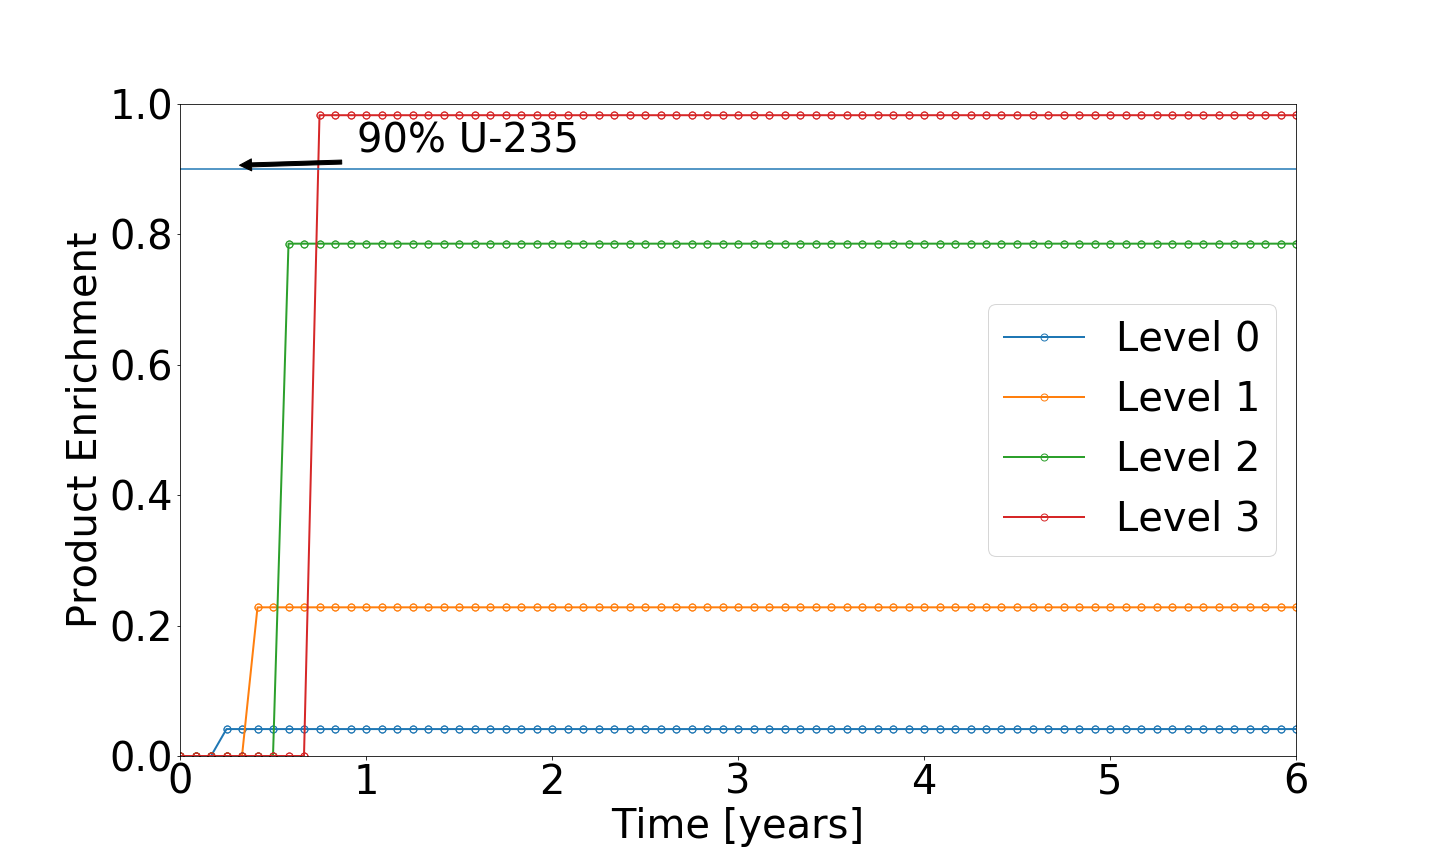
\includegraphics[scale=0.17]{NR_case1}
        \caption{No tails recycling}
        \label{sfig:case1_NR}
    \end{subfigure}%
    \begin{subfigure}[t]{0.45\textwidth}
        \centering
        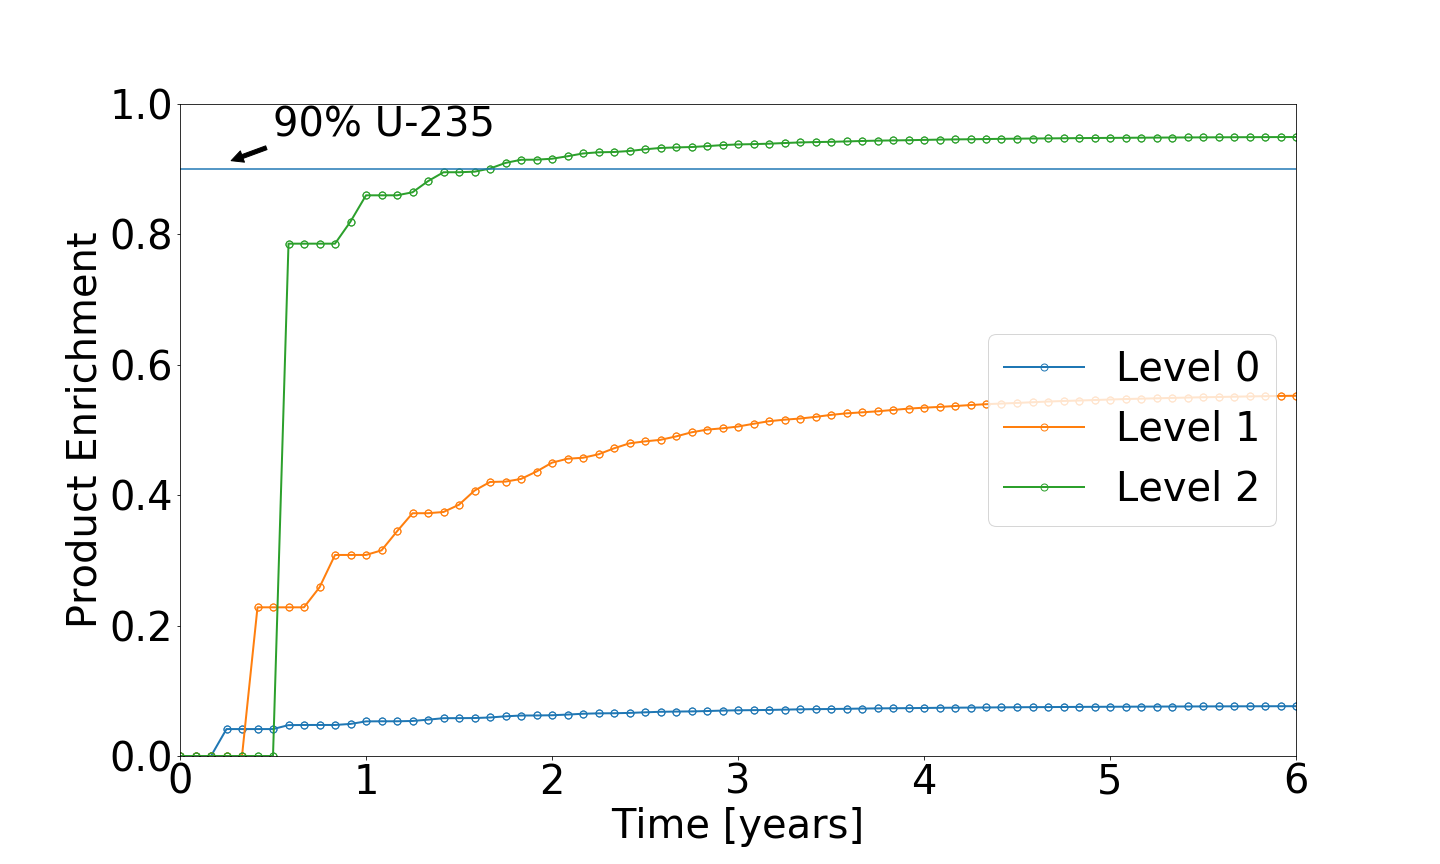
\includegraphics[scale=0.17]{R_case1}
        \caption{Tails recycling}
        \label{sfig:case1_R}
    \end{subfigure}
    \caption{Evolution of the product assays at each level with considering
    misuse model A, with (right) and without recycling (left).}
    \label{fig:case1}
\end{figure}


\begin{figure}[h!]
    \centering
    \begin{subfigure}[t]{0.45\textwidth}
        \centering
        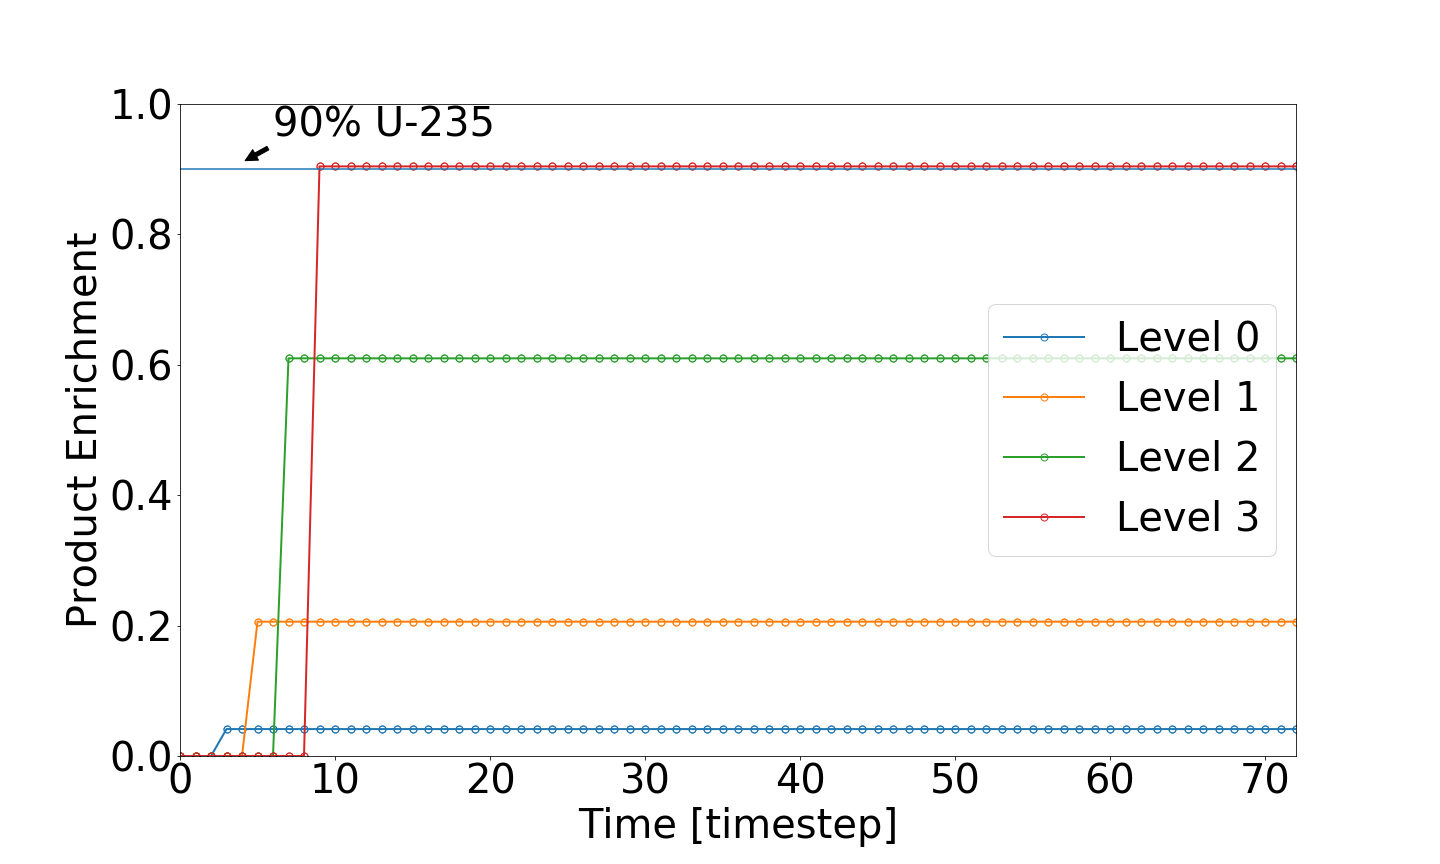
\includegraphics[scale=0.17]{NR_case2}
        \caption{No tails recycling}
        \label{sfig:case2_NR}
    \end{subfigure}%
    \begin{subfigure}[t]{0.45\textwidth}
        \centering
        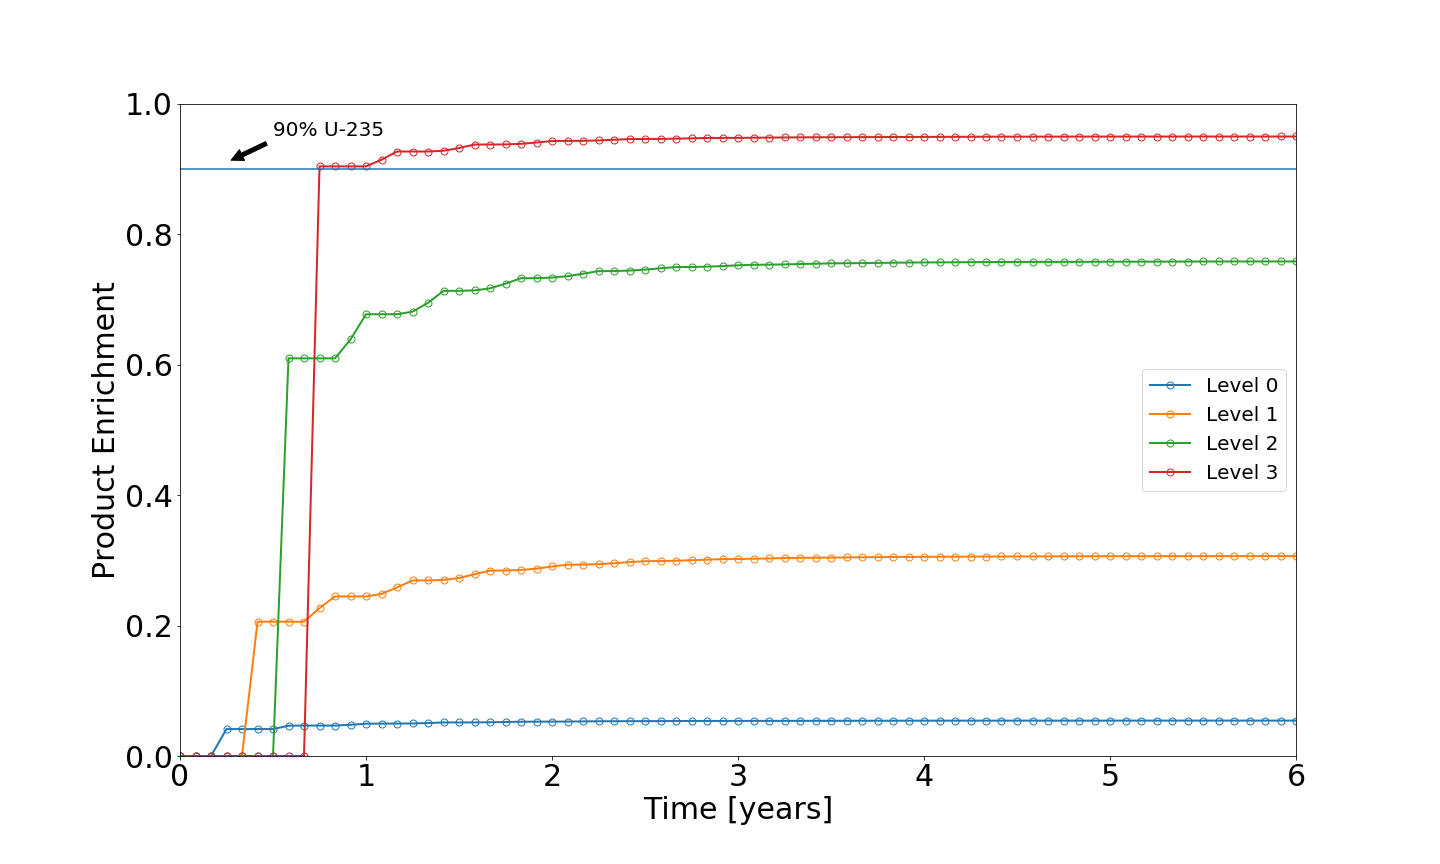
\includegraphics[scale=0.17]{R_case2}
        \caption{Tails recycling}
        \label{sfig:case2_R}
    \end{subfigure}
    \caption{Evolution of the product assays at each level with considering
    misuse model B, with (right) and without recycling (left).}
    \label{fig:case2}
\end{figure}

\subsection{Tails recycling}

As shown in Figures \ref{sfig:case1_R}, \ref{sfig:case2_R} and
\ref{sfig:case3_R}, recycling the tails increases the overall product assay at
all the different levels. As the tails assay of a level $n+1$ is always higher than
the product assay of the level $n-1$, recycling the tails of level $n+1$ will
consequently increase the feed assay of level $n$ (see Table \ref{tab:level}).
Moreover, with an increased feed assay, tails and product assays increase as
well, increasing de facto the feed assays of respectively cascade levels $n-1$
and $n+1$, etc.  This effect reduces the number of cascade levels required to reach
\gls{HEU} in case A and C.

\begin{figure}[h!]
    \centering
    \begin{subfigure}[t]{0.45\textwidth}
        \centering
        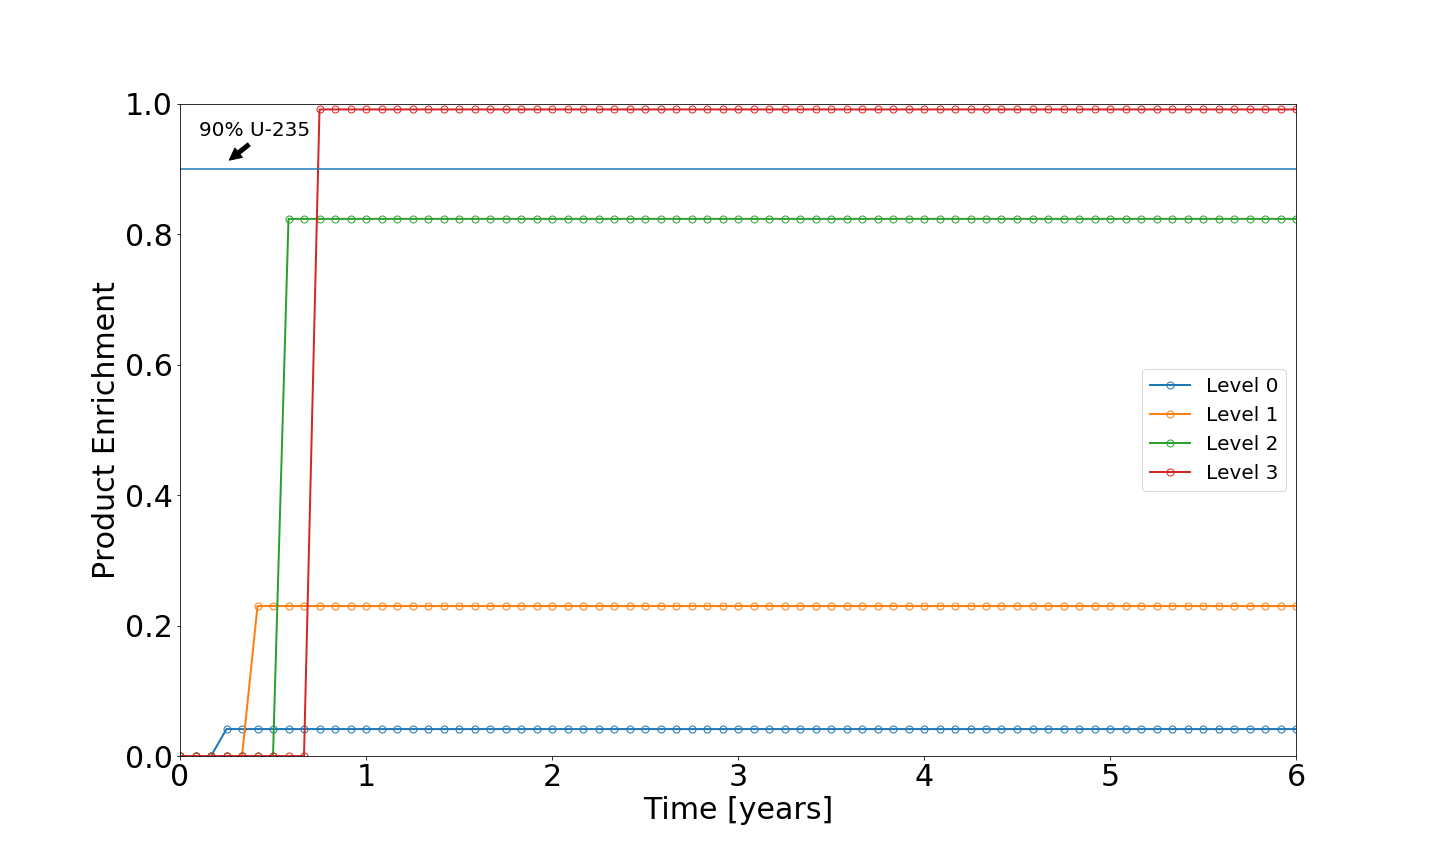
\includegraphics[scale=0.17]{NR_case3}
        \caption{No tails recycling}
        \label{sfig:case3_NR}
    \end{subfigure}%
    \begin{subfigure}[t]{0.45\textwidth}
        \centering
        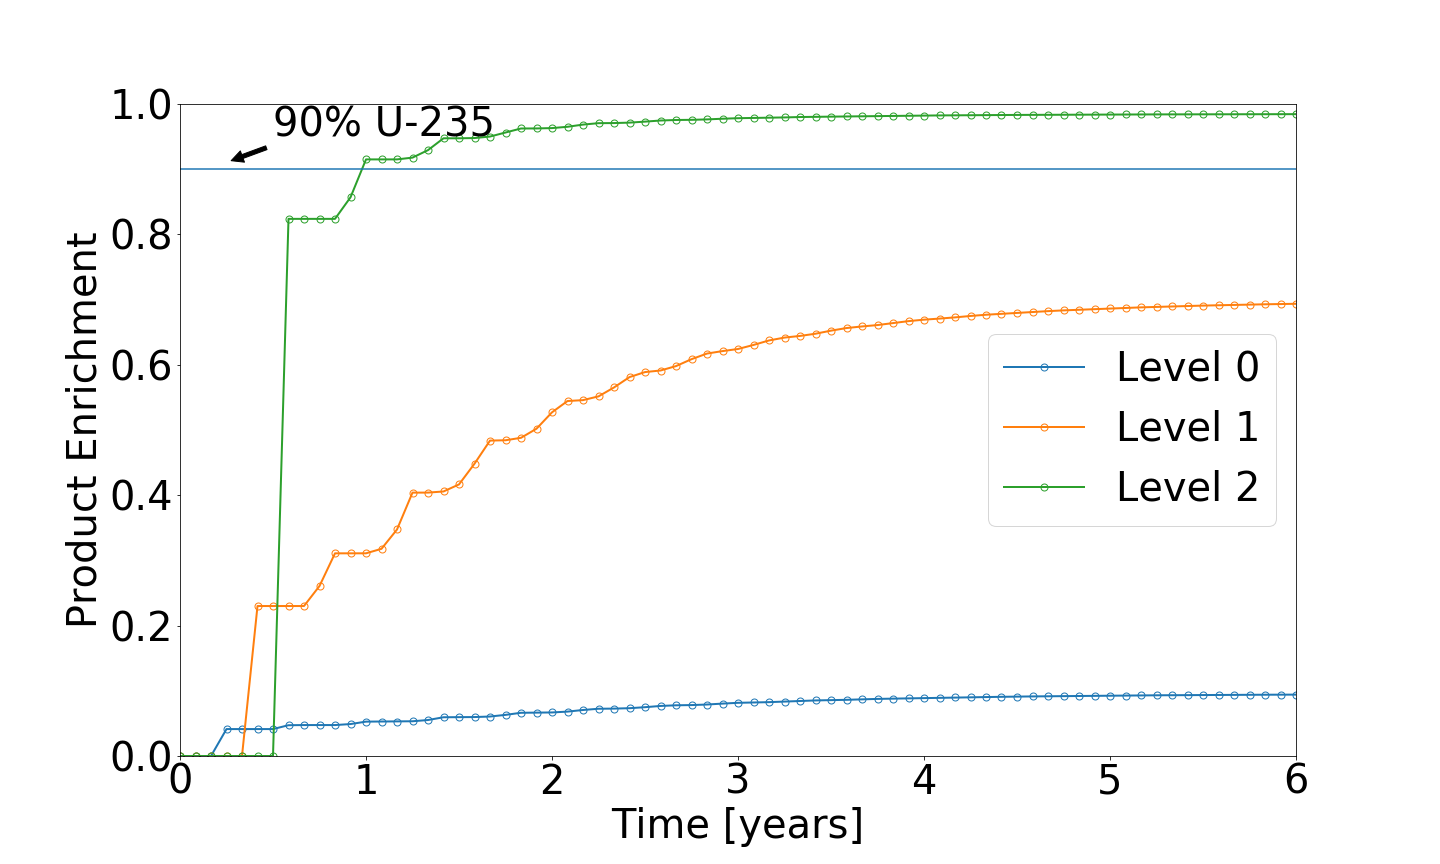
\includegraphics[scale=0.17]{R_case3}
        \caption{Tails recycling}
        \label{sfig:case3_R}
    \end{subfigure}
    \caption{Evolution of the product assays at each level with considering
    misuse model C, with (right) and without recycling (left).}
    \label{fig:case3}
\end{figure}



\subsection{\gls{HEU} Production}

As shown in Figure \ref{fig:HEU_rate}, recycling increases the final \gls{HEU}
production rate, from $2$ to almost $20$ kg/y when using model A and C, and from
$17$ to $38$ kg/y with the model B. For the reference calculation where all the
available cascades are used within a single large cascade design for direct
\gls{HEU} production, the \gls{HEU} production rate is slightly over $50$ kg/y.


As Model A and C, relies on maintaining the cut values at each stages of the
cascade and share the same number of levels, have the exact same cascade
repartition across the different levels and the same \gls{HEU} production rate.

\begin{figure}[h!] % replace 't' with 'b' to force it to be on the bottom
    \centering
    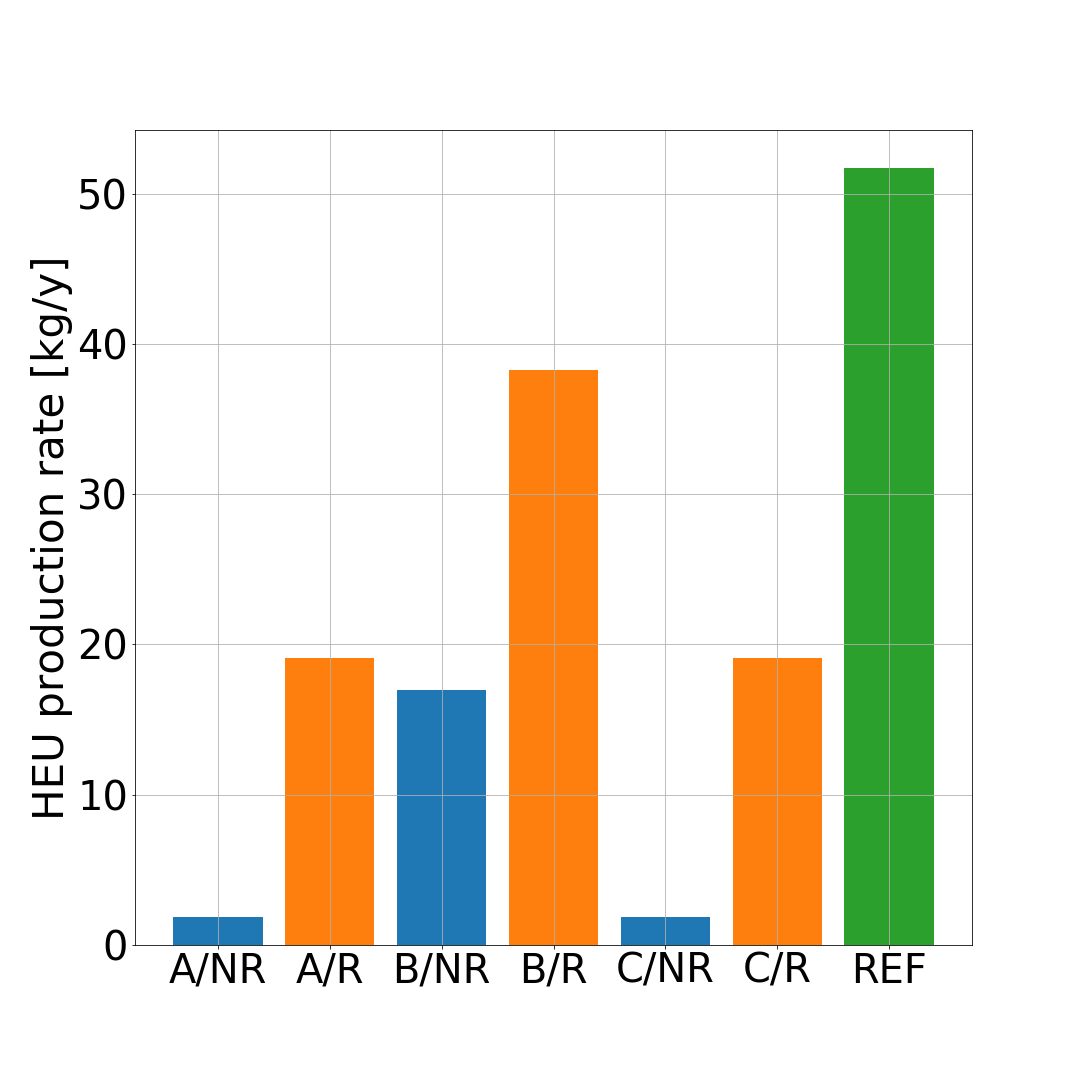
\includegraphics[scale=0.25]{HEU_prod_rate}
    \caption{Production rate at equilibrium for the different model
        configurations, the case without tails recycling (blue), with tails
        recycling (orange), and the reference one (green). A-B-C represent
        the model used, and NR-R the case without tails recycling and the case
        with tails recycling, respectively.}
    \label{fig:HEU_rate}
\end{figure}
